\section{Parsing}
The parser reads tokens generated by the scanner and generates phrases according to a context free grammar file which it then checks are syntactically correct. If there is an error it either reports it, attempts to repair it (to create a syntactically valid program), or tries to recover from the error in order to continue parsing. A parser is typically created through declarative programming. The results of parsing should also be, beside verifying the syntax of an program is valid, to create an abstract syntax tree.

%Parsing is a process where it analyses a string of symbols in a computer language and then trying to understand the meaning of the data that has been constructed. Which can then be made into a parse tree because the parsing understand the relationship by how the string of symbols must be understood. 
%This section will explain on what parsing is, how it works and what kind of different parsing methods exist. 

\subsection{Top-down and bottom-up parsing}
When constructing a parser, one of two strategies is usually used to recognize and construct tokens based on the context free grammar of the language, namely top-down parsing and bottom-up parsing.\\

Given a starting symbol and a set of rules, a top down parser will start reading its input as a long line of tokens from a lexer. In general, the tokens are read from left to right\footnote{Unless your source language is a language that writes from right to left, of course}, and are afterwards derived from the starting symbol using a leftmost-derivation of the non-terminals through the grammatical rules.

A parse tree represents an ordered structures of data nodes in a hierarchical way, where the nodes above are the parent nodes and the nodes under the parent nodes are the child nodes. It is constructed by a grammer or in this case for the project, a context-free-grammar \\
\begin{figure}[H]
\centering
\frame{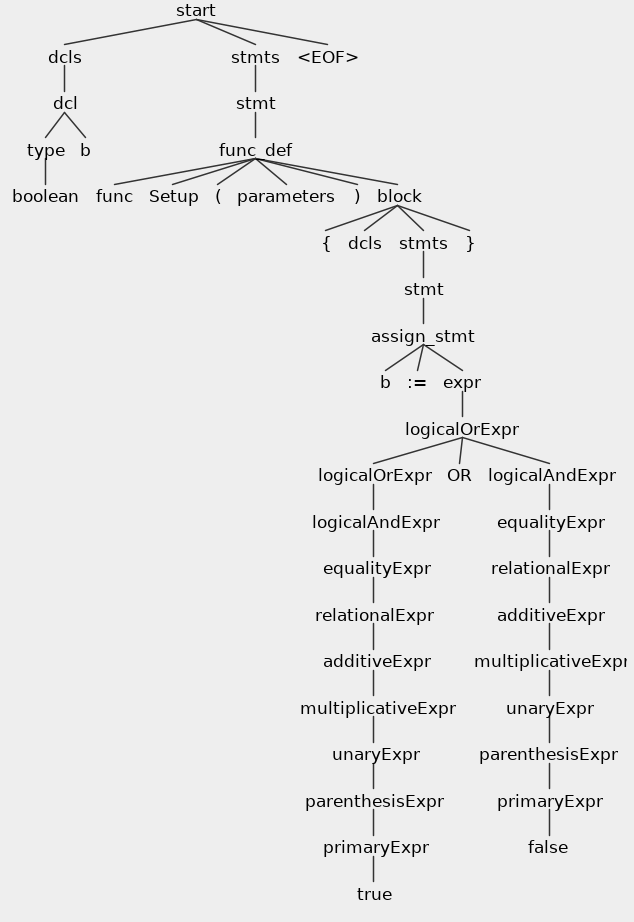
\includegraphics[width=0.7\textwidth]{figures/parse_tree_example.png}}
\caption{Parse tree example}
\label{exampleparse}
\end{figure}

The picture above shows a parse tree, where the highest node, which is A will have 2 child nodes which is B and C. It will than traverse further down until it reaches an end.
The top-down parsing is where the highest node of the parse tree will recognize the detail and from there on go down the parse tree until it hits and recognize the lowest part of the parse tree, which is the most lowest node, but it also reads the leftmost node first before going further down. Leftmost node means that you always start at the left non-terminal first and vice versa. We use top-down parsing when you want to create a hypothetical parsing tree with unknown data relationship, because the parsing tree would be testable to see if the hypothetical unknown data relationship could work together. The top-down parsing uses the LL(1) parsing, which will be explained later\cite{conceptsOfProgrammingLanguages}. 
\\
The buttom-up parsing is where the lowest  part of the parse tree will recognize the smallest part detail first and then go up from there until it hits and recognize the most abstract detail. The buttom-up parsing uses the LR(1) parsing technique unlike the top-down parsing and it scans the right most element first\cite{conceptsOfProgrammingLanguages}. 

\subsection*{LL(k) parsing}
The LL parser (Left to right and left most derivation) is a parser that parses its input from left to right while using a top-down parsing technique. In LL(k) the amount of k is to see how far it has to look ahead.\cite{conceptsOfProgrammingLanguages}


\subsection*{LR(1) parsing}
The LR parser (Left to right and right most derivation) is a parser that parses its input from left to right, but unlike the LL(k) parser, the LR parser uses a buttom-up parsing technique and produces a right most derivation. Just as the LL(k) the the k in the LL(k) defines the amount of tokens the LR will look ahead for\cite{LL-LR-Difference}. 

\subsection*{LALR(1) parsing}
The LALR(k) parser (Look ahead, left to right and right most derivation) is a parser that works the same way as the LR(k) parser, but the difference is that unlike the LR(k) parser the LALR(k) cannot do a backtracking, which is essential an algorithm for the parser to find potential candidates to that maybe can be a solution. If the algorithm finds the potential candidate to be a failure it would go back again to find another potential candidate for the solution. That means that he LALR(k) parser can only look ahead, which makes sense since the parser is by definintion LA(Look ahead)\cite{crafting-a-compiler}.
%Skal have review på LALR siden den forvirre mig. 

\subsection*{Table driven LL(K) parsing}
The table driven LL(k) parser uses a similarity analysis to the genereated grammar so that when it starts with pushing the start symbol into the stack, the parser would try and find match of symbols from the input and when found put the symbol into the top of the stack\cite{crafting-a-compiler}. This is good for when you have a code that is very big and want the parsing to be automatically by using a stack.

\subsection*{Recursive descent parser} 
The recursive descent parser is a top-down parser that is built from a collection of subprograms that each produces its own top-down parse tree generator. The subprograms in itself are recursive and the recursive descent parser will only create one subprogram for every non-terminal it can find in the user generated grammar. \cite{conceptsOfProgrammingLanguages}. 
